%% bare_jrnl.tex
%% V1.4b
%% 2015/08/26
%% by Michael Shell
%% see http://www.michaelshell.org/
%% for current contact information.
%%
%% This is a skeleton file demonstrating the use of IEEEtran.cls
%% (requires IEEEtran.cls version 1.8b or later) with an IEEE
%% journal paper.
%%
%% Support sites:
%% http://www.michaelshell.org/tex/ieeetran/
%% http://www.ctan.org/pkg/ieeetran
%% and
%% http://www.ieee.org/

%%*************************************************************************
%% Legal Notice:
%% This code is offered as-is without any warranty either expressed or
%% implied; without even the implied warranty of MERCHANTABILITY or
%% FITNESS FOR A PARTICULAR PURPOSE! 
%% User assumes all risk.
%% In no event shall the IEEE or any contributor to this code be liable for
%% any damages or losses, including, but not limited to, incidental,
%% consequential, or any other damages, resulting from the use or misuse
%% of any information contained here.
%%
%% All comments are the opinions of their respective authors and are not
%% necessarily endorsed by the IEEE.
%%
%% This work is distributed under the LaTeX Project Public License (LPPL)
%% ( http://www.latex-project.org/ ) version 1.3, and may be freely used,
%% distributed and modified. A copy of the LPPL, version 1.3, is included
%% in the base LaTeX documentation of all distributions of LaTeX released
%% 2003/12/01 or later.
%% Retain all contribution notices and credits.
%% ** Modified files should be clearly indicated as such, including  **
%% ** renaming them and changing author support contact information. **
%%*************************************************************************

%command to make pretty c++

\documentclass[journal]{IEEEtran}
\usepackage{amsmath}
\usepackage{fancyvrb}
% If IEEEtran.cls has not been installed into the LaTeX system files,
% manually specify the path to it like:
% \documentclass[journal]{../sty/IEEEtran}

% (uncomment the ones you want to load)

% *** MISC UTILITY PACKAGES ***
%
%\usepackage{ifpdf}
% Heiko Oberdiek's ifpdf.sty is very useful if you need conditional
% compilation based on whether the output is pdf or dvi.
% usage:
% \ifpdf
%   % pdf code
% \else
%   % dvi code
% \fi
% The latest version of ifpdf.sty can be obtained from:
% http://www.ctan.org/pkg/ifpdf
% Also, note that IEEEtran.cls V1.7 and later provides a builtin
% \ifCLASSINFOpdf conditional that works the same way.
% When switching from latex to pdflatex and vice-versa, the compiler may
% have to be run twice to clear warning/error messages.


% *** CITATION PACKAGES ***
%
%\usepackage{cite}
% cite.sty was written by Donald Arseneau
% V1.6 and later of IEEEtran pre-defines the format of the cite.sty package
% \cite{} output to follow that of the IEEE. Loading the cite package will
% result in citation numbers being automatically sorted and properly
% "compressed/ranged". e.g., [1], [9], [2], [7], [5], [6] without using
% cite.sty will become [1], [2], [5]--[7], [9] using cite.sty. cite.sty's
% \cite will automatically add leading space, if needed. Use cite.sty's
% noadjust option (cite.sty V3.8 and later) if you want to turn this off
% such as if a citation ever needs to be enclosed in parenthesis.
% cite.sty is already installed on most LaTeX systems. Be sure and use
% version 5.0 (2009-03-20) and later if using hyperref.sty.
% The latest version can be obtained at:
% http://www.ctan.org/pkg/cite
% The documentation is contained in the cite.sty file itself.


% *** GRAPHICS RELATED PACKAGES ***
%
\ifCLASSINFOpdf
  \usepackage[pdftex]{graphicx}
  % declare the path(s) where your graphic files are
  % \graphicspath{{../pdf/}{../jpeg/}}
  % and their extensions so you won't have to specify these with
  % every instance of \includegraphics
  % \DeclareGraphicsExtensions{.pdf,.jpeg,.png}
\else
  % or other class option (dvipsone, dvipdf, if not using dvips). graphicx
  % will default to the driver specified in the system graphics.cfg if no
  % driver is specified.
  % \usepackage[dvips]{graphicx}
  % declare the path(s) where your graphic files are
  % \graphicspath{{../eps/}}
  % and their extensions so you won't have to specify these with
  % every instance of \includegraphics
  % \DeclareGraphicsExtensions{.eps}
\fi
% graphicx was written by David Carlisle and Sebastian Rahtz. It is
% required if you want graphics, photos, etc. graphicx.sty is already
% installed on most LaTeX systems. The latest version and documentation
% can be obtained at: 
% http://www.ctan.org/pkg/graphicx
% Another good source of documentation is "Using Imported Graphics in
% LaTeX2e" by Keith Reckdahl which can be found at:
% http://www.ctan.org/pkg/epslatex
%
% latex, and pdflatex in dvi mode, support graphics in encapsulated
% postscript (.eps) format. pdflatex in pdf mode supports graphics
% in .pdf, .jpeg, .png and .mps (metapost) formats. Users should ensure
% that all non-photo figures use a vector format (.eps, .pdf, .mps) and
% not a bitmapped formats (.jpeg, .png). The IEEE frowns on bitmapped formats
% which can result in "jaggedy"/blurry rendering of lines and letters as
% well as large increases in file sizes.
%
% You can find documentation about the pdfTeX application at:
% http://www.tug.org/applications/pdftex


% *** MATH PACKAGES ***
%
%\usepackage{amsmath}
% A popular package from the American Mathematical Society that provides
% many useful and powerful commands for dealing with mathematics.
%
% Note that the amsmath package sets \interdisplaylinepenalty to 10000
% thus preventing page breaks from occurring within multiline equations. Use:
%\interdisplaylinepenalty=2500
% after loading amsmath to restore such page breaks as IEEEtran.cls normally
% does. amsmath.sty is already installed on most LaTeX systems. The latest
% version and documentation can be obtained at:
% http://www.ctan.org/pkg/amsmath


% *** SPECIALIZED LIST PACKAGES ***
%
%\usepackage{algorithmic}
% algorithmic.sty was written by Peter Williams and Rogerio Brito.
% This package provides an algorithmic environment fo describing algorithms.
% You can use the algorithmic environment in-text or within a figure
% environment to provide for a floating algorithm. Do NOT use the algorithm
% floating environment provided by algorithm.sty (by the same authors) or
% algorithm2e.sty (by Christophe Fiorio) as the IEEE does not use dedicated
% algorithm float types and packages that provide these will not provide
% correct IEEE style captions. The latest version and documentation of
% algorithmic.sty can be obtained at:
% http://www.ctan.org/pkg/algorithms
% Also of interest may be the (relatively newer and more customizable)
% algorithmicx.sty package by Szasz Janos:
% http://www.ctan.org/pkg/algorithmicx


% *** ALIGNMENT PACKAGES ***
%
%\usepackage{array}
% Frank Mittelbach's and David Carlisle's array.sty patches and improves
% the standard LaTeX2e array and tabular environments to provide better
% appearance and additional user controls. As the default LaTeX2e table
% generation code is lacking to the point of almost being broken with
% respect to the quality of the end results, all users are strongly
% advised to use an enhanced (at the very least that provided by array.sty)
% set of table tools. array.sty is already installed on most systems. The
% latest version and documentation can be obtained at:
% http://www.ctan.org/pkg/array


% IEEEtran contains the IEEEeqnarray family of commands that can be used to
% generate multiline equations as well as matrices, tables, etc., of high
% quality.


% *** SUBFIGURE PACKAGES ***
%\ifCLASSOPTIONcompsoc
%  \usepackage[caption=false,font=normalsize,labelfont=sf,textfont=sf]{subfig}
%\else
%  \usepackage[caption=false,font=footnotesize]{subfig}
%\fi
% subfig.sty, written by Steven Douglas Cochran, is the modern replacement
% for subfigure.sty, the latter of which is no longer maintained and is
% incompatible with some LaTeX packages including fixltx2e. However,
% subfig.sty requires and automatically loads Axel Sommerfeldt's caption.sty
% which will override IEEEtran.cls' handling of captions and this will result
% in non-IEEE style figure/table captions. To prevent this problem, be sure
% and invoke subfig.sty's "caption=false" package option (available since
% subfig.sty version 1.3, 2005/06/28) as this is will preserve IEEEtran.cls
% handling of captions.
% Note that the Computer Society format requires a larger sans serif font
% than the serif footnote size font used in traditional IEEE formatting
% and thus the need to invoke different subfig.sty package options depending
% on whether compsoc mode has been enabled.
%
% The latest version and documentation of subfig.sty can be obtained at:
% http://www.ctan.org/pkg/subfig


% *** FLOAT PACKAGES ***
%
%\usepackage{fixltx2e}
% fixltx2e, the successor to the earlier fix2col.sty, was written by
% Frank Mittelbach and David Carlisle. This package corrects a few problems
% in the LaTeX2e kernel, the most notable of which is that in current
% LaTeX2e releases, the ordering of single and double column floats is not
% guaranteed to be preserved. Thus, an unpatched LaTeX2e can allow a
% single column figure to be placed prior to an earlier double column
% figure.
% Be aware that LaTeX2e kernels dated 2015 and later have fixltx2e.sty's
% corrections already built into the system in which case a warning will
% be issued if an attempt is made to load fixltx2e.sty as it is no longer
% needed.
% The latest version and documentation can be found at:
% http://www.ctan.org/pkg/fixltx2e


%\usepackage{stfloats}
% stfloats.sty was written by Sigitas Tolusis. This package gives LaTeX2e
% the ability to do double column floats at the bottom of the page as well
% as the top. (e.g., "\begin{figure*}[!b]" is not normally possible in
% LaTeX2e). It also provides a command:
%\fnbelowfloat
% to enable the placement of footnotes below bottom floats (the standard
% LaTeX2e kernel puts them above bottom floats). This is an invasive package
% which rewrites many portions of the LaTeX2e float routines. It may not work
% with other packages that modify the LaTeX2e float routines. The latest
% version and documentation can be obtained at:
% http://www.ctan.org/pkg/stfloats
% Do not use the stfloats baselinefloat ability as the IEEE does not allow
% \baselineskip to stretch. Authors submitting work to the IEEE should note
% that the IEEE rarely uses double column equations and that authors should try
% to avoid such use. Do not be tempted to use the cuted.sty or midfloat.sty
% packages (also by Sigitas Tolusis) as the IEEE does not format its papers in
% such ways.
% Do not attempt to use stfloats with fixltx2e as they are incompatible.
% Instead, use Morten Hogholm'a dblfloatfix which combines the features
% of both fixltx2e and stfloats:
%
% \usepackage{dblfloatfix}
% The latest version can be found at:
% http://www.ctan.org/pkg/dblfloatfix


%\ifCLASSOPTIONcaptionsoff
%  \usepackage[nomarkers]{endfloat}
% \let\MYoriglatexcaption\caption
% \renewcommand{\caption}[2][\relax]{\MYoriglatexcaption[#2]{#2}}
%\fi
% endfloat.sty was written by James Darrell McCauley, Jeff Goldberg and 
% Axel Sommerfeldt. This package may be useful when used in conjunction with 
% IEEEtran.cls'  captionsoff option. Some IEEE journals/societies require that
% submissions have lists of figures/tables at the end of the paper and that
% figures/tables without any captions are placed on a page by themselves at
% the end of the document. If needed, the draftcls IEEEtran class option or
% \CLASSINPUTbaselinestretch interface can be used to increase the line
% spacing as well. Be sure and use the nomarkers option of endfloat to
% prevent endfloat from "marking" where the figures would have been placed
% in the text. The two hack lines of code above are a slight modification of
% that suggested by in the endfloat docs (section 8.4.1) to ensure that
% the full captions always appear in the list of figures/tables - even if
% the user used the short optional argument of \caption[]{}.
% IEEE papers do not typically make use of \caption[]'s optional argument,
% so this should not be an issue. A similar trick can be used to disable
% captions of packages such as subfig.sty that lack options to turn off
% the subcaptions:
% For subfig.sty:
% \let\MYorigsubfloat\subfloat
% \renewcommand{\subfloat}[2][\relax]{\MYorigsubfloat[]{#2}}
% However, the above trick will not work if both optional arguments of
% the \subfloat command are used. Furthermore, there needs to be a
% description of each subfigure *somewhere* and endfloat does not add
% subfigure captions to its list of figures. Thus, the best approach is to
% avoid the use of subfigure captions (many IEEE journals avoid them anyway)
% and instead reference/explain all the subfigures within the main caption.
% The latest version of endfloat.sty and its documentation can obtained at:
% http://www.ctan.org/pkg/endfloat
%
% The IEEEtran \ifCLASSOPTIONcaptionsoff conditional can also be used
% later in the document, say, to conditionally put the References on a 
% page by themselves.


% *** PDF, URL AND HYPERLINK PACKAGES ***
%
%\usepackage{url}
% url.sty was written by Donald Arseneau. It provides better support for
% handling and breaking URLs. url.sty is already installed on most LaTeX
% systems. The latest version and documentation can be obtained at:
% http://www.ctan.org/pkg/url
% Basically, \url{my_url_here}.


% *** Do not adjust lengths that control margins, column widths, etc. ***
% *** Do not use packages that alter fonts (such as pslatex).         ***
% There should be no need to do such things with IEEEtran.cls V1.6 and later.
% (Unless specifically asked to do so by the journal or conference you plan
% to submit to, of course. )


% correct bad hyphenation here
\hyphenation{op-tical net-works semi-conduc-tor}


\begin{document}
%
% paper title
% Titles are generally capitalized except for words such as a, an, and, as,
% at, but, by, for, in, nor, of, on, or, the, to and up, which are usually
% not capitalized unless they are the first or last word of the title.
% Linebreaks \\ can be used within to get better formatting as desired.
% Do not put math or special symbols in the title.
\title{Developing a Parallel Raster Plugin\\For QGIS}
%
%
% author names and IEEE memberships
% note positions of commas and nonbreaking spaces ( ~ ) LaTeX will not break
% a structure at a ~ so this keeps an author's name from being broken across
% two lines.
% use \thanks{} to gain access to the first footnote area
% a separate \thanks must be used for each paragraph as LaTeX2e's \thanks
% was not built to handle multiple paragraphs
%

\author{Alex~Feurst,
        William~Hoffman,
        Charles~Kazer,
        and~Dr.~Arthur~Lembo}%

% note the % following the last \IEEEmembership and also \thanks - 
% these prevent an unwanted space from occurring between the last author name
% and the end of the author line. i.e., if you had this:
% 
% \author{....lastname \thanks{...} \thanks{...} }
%                     ^------------^------------^----Do not want these spaces!
%
% a space would be appended to the last name and could cause every name on that
% line to be shifted left slightly. This is one of those "LaTeX things". For
% instance, "\textbf{A} \textbf{B}" will typeset as "A B" not "AB". To get
% "AB" then you have to do: "\textbf{A}\textbf{B}"
% \thanks is no different in this regard, so shield the last } of each \thanks
% that ends a line with a % and do not let a space in before the next \thanks.
% Spaces after \IEEEmembership other than the last one are OK (and needed) as
% you are supposed to have spaces between the names. For what it is worth,
% this is a minor point as most people would not even notice if the said evil
% space somehow managed to creep in.



% The paper headers
%\markboth{Journal of \LaTeX\ Class Files,~Vol.~14, No.~8, August~2015}%
%{Shell \MakeLowercase{\textit{et al.}}: Bare Demo of IEEEtran.cls for IEEE Journals}
% The only time the second header will appear is for the odd numbered pages
% after the title page when using the twoside option.
% 
% *** Note that you probably will NOT want to include the author's ***
% *** name in the headers of peer review papers.                   ***
% You can use \ifCLASSOPTIONpeerreview for conditional compilation here if
% you desire.


% If you want to put a publisher's ID mark on the page you can do it like
% this:
%\IEEEpubid{0000--0000/00\$00.00~\copyright~2015 IEEE}
% Remember, if you use this you must call \IEEEpubidadjcol in the second
% column for its text to clear the IEEEpubid mark.


% use for special paper notices
%\IEEEspecialpapernotice{(Invited Paper)}

% For align

% make the title area
\maketitle

% As a general rule, do not put math, special symbols or citations
% in the abstract or keywords.
\begin{abstract}
    Geographic Information Systems (GIS) are used in many different fields
    to analyze spatial data and plan accordingly. Geographic data has been
    growing in size exponentially, and while some GIS tools to analyze this
    data have been created, usage and efficiency have been lagging behind. The
    advent of massively parallel computing, specifically the availability of
    GPU programming, have made a more efficient solution possible since most
    GIS calculations are embarrassingly parallel. QGIS is an open source GIS
    platform that has gained much traction in the computational geography
    community. We created a QGIS plugin that leverages GPUs to increase
    calculation speed on large data sets. We developed this plugin with
    the geography community in mind, using Python to make code easy to read,
    portable, and modifiable.
\end{abstract}

% Note that keywords are not normally used for peerreview papers.
\begin{IEEEkeywords}
    CUDA, Parallel Processing, GIS
\end{IEEEkeywords}



% For peer review papers, you can put extra information on the cover
% page as needed:
% \ifCLASSOPTIONpeerreview
% \begin{center} \bfseries EDICS Category: 3-BBND \end{center}
% \fi
%
% For peerreview papers, this IEEEtran command inserts a page break and
% creates the second title. It will be ignored for other modes.
\IEEEpeerreviewmaketitle



\section{Background and Introduction}
% The very first letter is a 2 line initial drop letter followed
% by the rest of the first word in caps.
% 
% form to use if the first word consists of a single letter:
% \IEEEPARstart{A}{demo} file is ....
% 
% form to use if you need the single drop letter followed by
% normal text (unknown if ever used by the IEEE):
% \IEEEPARstart{A}{}demo file is ....
% 
% Some journals put the first two words in caps:
% \IEEEPARstart{T}{his demo} file is ....
% 
% Here we have the typical use of a "T" for an initial drop letter
% and "HIS" in caps to complete the first word.
\IEEEPARstart{W}{e} are three undergraduates from across the country that came
together in a National Science Foundation Research for Undergraduates for an 
educational experience in professional style research. Dr. Lembo came up with
the project that the three of us researched.Parallel computing has been adopted
in many fields to improve computation efficiency. Although many analytics in 
Geographic Information Systems (GIS) are embarrassingly parallelizable, 
parallel computing has yet to be largely adopted in the community. We've 
developed open source software for parallel raster calculations to spur the GIS
community to adopt parallel computing practices. This plugin was built for the
popular, open source GIS software QGIS, and performs parallel slope, aspect 
and/or hillshade calculations on an arbitrary raster file.  We've implemented 
the plugin using Python and PyCUDA, an open source library for Python built on 
top of the CUDA programming language for \textsc{NVIDIA} graphics cards. Our
current results indicate a efficient, scalable improvement over similar serial
calculations.

\section{Related Work} \label{related}
The idea of using parallel processing in GIS had been around for a long time
\cite{healy}, but only recently has been seriously considered.  Similar work on
creating open source, accessible parallel GIS tools has been done in the past,
though no one method has been widely adopted. The authors of \cite{guan}
created a C++ library for parallel raster file processing, though this only
uses CPU parallelization. \cite{benedicic} created a GRASS GIS module based on
cluster computing designed to predict radio-coverage. \cite{Cheng} used 
parallelism to try and improve the computing i/o for digital terrain analysis.
GIS algorithms have also been parallelized over clusters of machines rather
than just CPU parallelization, such as in \cite{huang}.  \cite{hpc_cuda} 
developed a C++ library for simple raster calculations using CUDA as an 
extension to the proprietary ArcGIS software. Implementation with CUDA and
GPUs was extended upon in \cite{Xu} to test the efficiency of a string
matching algorithm. GPUs and CUDA were also used in \cite{Saha} to apply
brightening and darkening filters. Other members of the computer science 
community in recent years have started testing methods to speed up the 
computing process on large scale data and some have used GPUs as well. 
\cite{Gaurav} tested a varity of GPU calculation methods and speed comparisons 
between all of them for future projects. GPUs were used on large scale pixel 
data in \cite{Wadbro} to show the usfulness of GPUs on big data. \cite{Zhang} 
used GPUs with grids of raster data to do speed comparisons with 
traditional search methods done on the CPU vs the GPU. Another highly 
repetative process was tested in \cite{Yang} and \cite{Martínez-Frutos} 
with the testing of Sliding Windows Operations over CPUs and GPUs for 
compariaon. GPUs were used in comparison with Intel's Many Integrated Core
from \cite{Shi} to predict better efficiency for future spatial data 
problems. Large scale Digital Elevation Models were used in \cite{Tabik} by 
using solar measurements and angle data through a CPU-GPU heterogeneous 
system. We want to progress the work of these works to be more accessible 
to the GIS community.

\section{Problem Outline} \label{problem}
    \subsection{Computational Challenges}
    GIS analytics perform many independent calculations on extremely large data
    sets. This proves problematic due to the memory limitations of a single
    machine, and the massive amount of calculations that need to be run. Data sets 
    typically analyzed by GIS can be in the terabyte (TB) realm. With
    most computers only having memory capabilities in the gigabyte (GB) range,
    steps must be taken to work around running out of memory. Both the large size
    of data sets and the requirement that each piece of data be analyzed separately
    slows down processing time dramatically. Input from and output to data sets
    and memory have proven to be a major component to the slow down.  However,
    performing the large amount of independent calculations through serial
    programming also bogs down the process. Our goal is to build a system that
    maximizes Input/Output (I/O) throughput as well as reduce computation time
    through parallelism.

    \subsection{Ease of Use}
    Use of parallelism in GIS has been explored in the past, yet despite its proven
    benefits over serial calculation, the GIS community has been slow to adopt
    parallel computation. This is largely because the introduction of parallelism
    makes code much more difficult to read and write. Parallelism is something that
    many experienced programmers struggle with, let alone the many members of the
    GIS community who have little to no experience with programming. With this in
    mind, we have tried to write the parallel processing tools presented here in a
    simple, easy to modify way without giving up the power of parallelism
    altogether.  For those who don't even want exposure to any source code, we
    have provided a plugin to the popular, open source GIS, QGIS with a simple
    GUI that runs the parallel code.


\section{Methods} \label{methods}
    \begin{figure}
        \includegraphics[width=\linewidth]{model2.png}
        \caption{Main work flow model.}
        \label{model}
    \end{figure}
    \subsection{Scheduler Model}
    The previous work done in \cite{hpc_cuda} revealed that the greatest
    hindrance to performance in GPU based GIS calculations is the transfer of
    data from disk to main memory, and then from main memory to GPU memory.
    Memory transfer must occur four times for each GPU job, loading from disk
    to main memory, loading from main memory to GPU memory, and then copying
    results from GPU memory back to main memory, and then to disk.  Further
    compounding the problem is that GPU memory is typically more limited than
    main memory, so multiple copies from main memory are required for files
    larger than the available memory on the GPU. Thus we have designed our
    work flow to try to mitigate the effects of the I/O bottleneck.

    Figure \ref{model} shows our design model. There are three main processes,
    the data loader, the data saver, and GPU manager. Broadly, the data loader
    is responsible for loading data from disk and formatting from its initial
    file type, the data saver is responsible for compressing and saving data
    back to disk, and the GPU manager is responsible for running GPU tasks,
    including copying data to and back from the GPU. The three processes are
    described in more detail in section \ref{implementation}. The three
    processes run independently, so data can be loaded from disk, calculations
    can be performed on the GPU, and data can be saved to disk all
    simultaneously.  This provides parallelism both on the CPU for I/O, and on
    the GPU for calculations, improving overall computation time.
    
    \subsection{GPU Kernel}
    The GPU kernel, the algorithm that is executed on the GPU in parallel, is
    designed to perform analysis on individual cells in a raster file based on
    a 3x3 grid around the cell. The kernel was designed to be modular so that
    any kind of calculation can be done based on the 3x3 grid of neighbors. A
    user simply needs to write the desired calculation, and the rest of the
    kernel was written ensure that all of the correct data is available on any
    given thread for a 3x3 grid calculation.  The kernel uses a grid striding
    loop for flexibility and
    efficiency\cite{grid_stride}.

    \subsection{GIS Algorithms}
    The algorithms we implemented utilize a 3x3 cell neighborhood around each 
    calculated cell. 
    \begin{figure}
        \center
        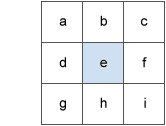
\includegraphics[width=2in]{GISgrid.jpg}
        \caption{3x3 cell neighborhood}
        \label{GIS grid}
    \end{figure}
    This 3x3 grid is used to calculate the rate of change from east to west
    \(\frac{dz}{dx}\) and the rate of change from north to south
    \(\frac{dz}{dy}\). These are found as follows:
    \[\frac{dz}{dx} = ((c + 2f + i) - (a + 2d + g) / (8 * x\_cellsize)\]
    \[\frac{dz}{dy} = ((g + 2h + i) - (a + 2b + c)) / ( 8 * y\_cellsize)\]
    where the letters correspond to the positions in \ref{GIS grid}.

    These rates of change are used to calculate slope, aspect and hillshade.
    Slope is the maximum rate of change in elevation between the cell and its
    neighbors. The lower the slope value the flatter the land is. It is
    calculated with the following formula:
    \[Slope = ATAN\Bigg(\sqrt{\Big(\frac{dz}{dx}\Big)^{2} + \Big(\frac{dz}{dy}\Big)^{2}}~\Bigg)\]

    Aspect identies the direction of the downslope. Aspect is found using
    %conditional steps and is calculated in degrees, which can be converted to
    %radians.
    the following formula:
    \[Aspect = 57.29578 * ATAN2\bigg(\frac{dz}{dy}, -\frac{dz}{dx}\bigg)\]

    Hillshade is the hypothetical illumination of the surface when the sun is
    at a specific height and angle in the sky. It is a more complex algorithm
    and relies on slope and aspect being calculated in addition to finding the
    illumination angle zenith (abbreviated \(zen\)) and illumination
    direction azimuth (abbreviated \(azm\)). We have defaulted these values
    to 45 degrees and 315 degrees respectively.
    \begin{align*}
        Hillshade =& ~ 255.0 ((COS(zen) * COS(slope)) ~ +  \\
                   &(SIN(zen) * SIN(slope) * COS(azm - aspect))
    \end{align*}

    \subsection{QGIS Integration}
    We have constructed a QGIS plugin, depicted in figure \ref{gui} which uses
    our data processing pipeline and presents a simple GUI where a user can
    select an input file, output file, and operations to perform. This way,
    once the plugin is installed, a user need not even interact with the
    command line, or learn to use a new piece of software in order to perform
    GPU calculations. We have also tried to allow users to load data directly
    from QGIS rather than from disk, but this feature is still unstable.
    \begin{figure}
        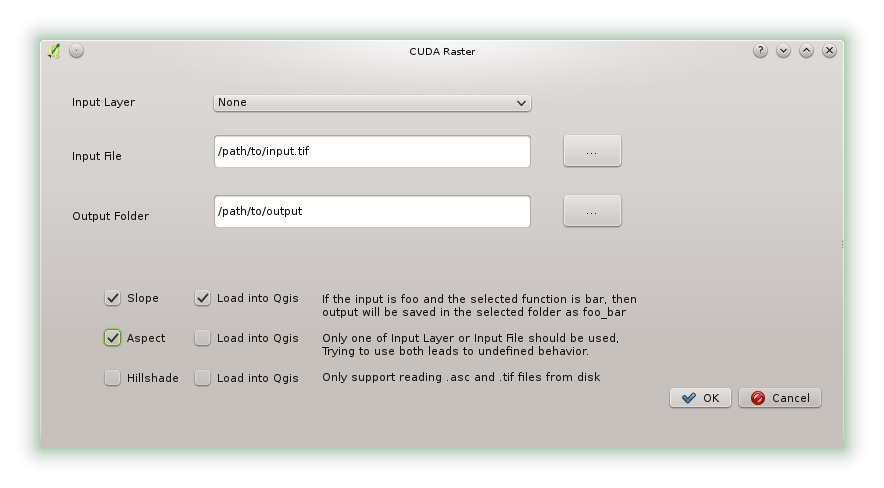
\includegraphics[width=\linewidth]{gui.png}
        \caption{Snapshot of plugin GUI.}
        \label{gui}
    \end{figure}

\section{Implementation} \label{implementation}
    Our program is implemented primarily in Python 2.7. We chose to write the
    program in Python because it is relatively easy to read and write, and also
    allowed us to produce shorter, more compact code than the C or C++ code
    typically used with CUDA.  Although Python is slower than C or C++, we
    thought the readability trade-off was worth it so that others in the GIS
    community could read, test, and modify our code. In order to still get as
    much efficiency as possible, we used the GDAL libraries, Numpy, and PyCUDA
    \cite{pycuda_1} \cite{pycuda_2}. PyCUDA serves as a wrapper for CUDA C that
    handles many of the ugly details of memory allocation and transfer to the
    GPU. Unfortunately, kernel code to be executed on the GPU must still be
    written in C. 
    
    \begin{align*}
        While there is input or output
	\\DataLoader reads input into blocks
	\\Blocks of raw data are sent to GPUManager
	\\GPUManager sends raw data to GPU
	\\GPU computes raw as slope and/or aspect and/or hillshade
	\\GPUManager takes back computed data from GPU
	\\Computed data blocks are sent to DataSaver
	\\DataSaver writes computed blocks to output files
	End While
    \end{align*}
    
    Our program's structure follows the model in figure \ref{model}. The
    following sections describe the implementation of each process.

    \subsection{Scheduler}
    The scheduler class starts and manages the other processes. It is
    responsible for parsing the desired input, functions, and output. It starts
    each other process and coordinates passing information between them. The
    scheduler also ensures that each other process terminates properly, and if
    not attempts to print useful information about which process caused the
    error. Although figure \ref{model} only depicts one saver, multiple
    functions can be computed on a single file loaded by the data loader, and
    the scheduler will generate a different saver to individually save each
    output.
    
    \begin{Verbatim}[frame=single, gobble=4]
    # join all threads
    while active_children():
      if  loader.exitcode != 0:
       print "Error encountered in loader"            
       calc.stop()
       for saver in savers:
        saver.stop()
       break
      if calc.exitcode != 0:
       loader.stop()
       for saver in savers:
        saver.stop()
       print "Error encountered in GPU"
       break
      sleep(1)    
    total = time() - start
    print "Total time: %d mins, %f secs" \
        % (total / 60, total % 60)
    \end{Verbatim}
    \break

    \subsection{Loader}
    The loader class reads data from a given input file and passes it into
    a pipe object, which goes to the GPU manager. We use the GDAL libraries to
    read files from disk because it is optimized on raster data files. The data is
    formatted row by row into Numpy arrays and then passed to the GPU manager.
    We chose to have a single row of data be our transfer unit because it makes
    both the loader and the GPU kernel easier to understand than if we tried to
    use two dimensional blocks of data. The loader class is also responsible
    for providing the GPU Manager and data saver file metadata, such as the
    dimensions of the raster and the area that each pixel represents.

    Originally, we pulled lines from the file with GDAL one by one, matching
    how we send one row at a time through the pipe. However, we found that this
    could be made more efficient if GDAL read more rows per read call, likely
    because fewer system calls are made that way. Empirically, the optimal number
    of rows to cache depends on the dimensions of the raster file. 30 rows seems
    to be a good starting point.

\begin{Verbatim}[frame=single, gobble=2]
   data = openRaster.read(0, line_num, 
	      cols, rows, buf_type=dataType)
   ext=struct.unpack(unpackVal*rows, data)
   for line in range(rows):
    output_pipe.send(float32(
	     ext[line*cols:][:cols]))
\end{Verbatim}

    The QGIS plugin version also supports reading raster data from a layer loaded
    into QGIS rather than from disk. When read this way, the loader uses the QGIS
    python API to load a Numpy array of a single row of data.

    \subsection{GPU Manager}
    The GPU manager is where the actual calculations on the data are performed,
    and where the bulk of the code exists. The manager functions by reading a
    page worth of data from the input pipe, performing GPU calculations on that
    page, then sending that through an output pipe to the data saver. Each page
    is sized to exactly fit a certain number of rows of data. The GPU manager
    is designed to be robust in that it bases all of its memory management on
    the GPU card of the system it runs on. Although the kernel code is somewhat
    complex, it is designed so that one could write any algorithm based on a
    3x3 grid of pixels to be plugged into the rest of the kernel code and calculated.

    The GPU manager starts by initializing the buffers which will be used to
    copy memory to and retrieve memory from the GPU. These are based on the
    available GPU memory when the process starts, so it should always saturate
    GPU memory. It then pre-compiles the GPU kernels for each requested
    calculation on the data. Finally, the manager enters the main processing loop
    where data is received and analyzed.

    Once the read buffer receives a page worth of data, it serially runs each
    requested kernel, copies the results back from the GPU, and sends the data
    for each kernel to a different saver. Each kernel is scheduled to run on
    as many GPU cores as possible, to minimize computation time.

    \begin{Verbatim}[frame=single, gobble=8]
        grd = (256,256)
        blk = (32,32,1)
        blocks = grd[0] * grd[1]
        threads = blk[0]*blk[1]*blk[2]
	# pixels per threas
        ppt = (rows * cols) / (threads * blocks)    

        # minimize work by each thread]
        while ppt < 3:
         grd = (grd[0] - 16,grd[1] - 16)
         blocks = grd[0] * grd[1]
         ppt = (rows * cols)/(threads * blocks)
        ppt = np.ceil(ppt)   
        
        #information struct passed to GPU
        stc = GPUStruct([
         (np.uint64, 'ppt', ppt),
         (np.float64, 'NODATA', NODATA),
         (np.uint64, 'ncols', cols),
         (np.uint64, 'nrows', rown),
         (np.uint64, 'npixels', rows*cols),
         (np.float32, 'cellSize', cellsize)
         ])

        stc.copy_to_gpu()
        #Call GPU kernel
        func(data_gpu, result_gpu, stc, blk, grd)
\end{Verbatim}

    \subsection{Saver}
    The data saver class takes the results of the calculations done in the GPU
    manager and saves them to disk. Similar to the data loader, the data saver
    uses the GDAL libraries to write multiple lines at a time to a Geotiff.
    Multiple savers can all run in parallel to save the ouputs of different
    functions.
\break
    \begin{Verbatim}[frame=single, gobble=4]
    try:
     for row in range(self.write_rows):
      np.put(out_arr[row], input_pipe.recv())
    except EOFError:
      print "Pipe closed unexpectedly"
       self.stop()
    # write out rows
    dataset.WriteArray(out_arr, 0, nrows)
\end{Verbatim}


    \subsection{QGIS Plugin}
    For QGIS, we implemented a simple GUI plugin that calls our code. The plugin
    was made using the QGIS plugin builder tool to generate all of the skeleton
    code and QT creator to design the GUI. The plugin takes input and output
    information from the user, then calls the scheduler on those parameters.

    Although there are a still a few issues, we also implemented loading data
    from a QGIs layer, rather than from disk. This separate version of the loader
    reads values using the QGIS API, so if QGIS has raster information cached in
    memory, it should load values faster than from disk. The QGIS loader still
    sends one row of data at a time through a pipe, so no changes are needed
    for it to work with the GPU manager or data saver.

\begin{Verbatim}[frame=single, gobble=7]
        layer = inputLayer
        ext = layer.extent()
        data = layer.dataProvider()
        ret_arr=[]
        for x in range(layer.width()):
            ret_arr.append(data.value(row,x))
        return float32(ret_arr)
\end{Verbatim}
    
\section{Analysis}
Timing our implementation for parallel hillshade and slope calculation from a raster file
against the standard serial methods used in QGIS has revealed the input and
output will be our biggest hurdle to overcome. Timing data can be seen in these
tables.

\vspace{.25in}
\pagebreak
\textbf{Hillshade timings}
\vspace{0.05in}

\begin{tabular}{ l | c | c }
    File Size & QGIS   & PyCUDA\\ \hline
    25 MB     & 5 secs & 3 secs\\ \hline
    200 Mb    & 15 secs & 6 secs\\ \hline
    1.5 GB    & 11 mins & 3 mins\\ \hline
    8 GB      & 45 mins & 30 mins
\end {tabular}

\vspace{.25in}
\textbf{Slope breakdown}
\vspace{0.05in}

\begin{tabular}{ l | c | c }
    Function    & QGIS & PyCUDA\\ \hline
    Input       & 2:00 & 1:55\\ \hline
    Computation & 5:00 & 1:00\\ \hline
    Output      & 2:00 & 2:20\\ \hline
    Total       & 9:00 & 3:35
\end {tabular}

\vspace{.25in}
\textbf{Hillshade breakdown}
\vspace{0.05in}

\begin{tabular}{ l | c | c }
    Function    & QGIS & PyCUDA\\ \hline
    Input       & 2:00 & 1:55\\ \hline
    Computation & 7:00 & 1:00\\ \hline
    Output      & 2:00 & 2:20\\ \hline
    Total       & 11:00 & 3:35
\end {tabular}
\vspace{0.25in}

The PyCUDA version is consistently faster than QGIS when calculating hillshade
for files of various sizes. The I/O bottleneck  can be seen in the input and
output sections of the second table. PyCUDA spends almost as much time dealing
with disk as QGIS does which limits the maximum speedup from using the GPU.
Output takes a much longer time because it has to wait for the GPU to pass data
to the saver before it can start saving to disk.  GPU computations, including
CPU based memory management took one ninth of the time required to do the
same thing in QGIS. Most of this time is spent sending or receiving data, once
the information is on the card the GPU finishes extremely quickly. Including
moving data to and from the card, the accumulated execution time for the GPU
was less than 2 seconds.  Both slope and hillshade are calculated in almost the
same time by the GPU, showing that it isn't being significantly taxed by the
more complicated formula and could easily do more work.  A process that
required hundreds or thousands of computations per element would be perfect for
adaptation onto GPU processing. Testing showed that even computing hillshade
several hundred times on each pixel didn't increase the time needed to finish.


\section{Conclusion}
We have developed a PyCUDA based, open source raster calculation tool that can
run either from the command line or as a plugin for QGIS. The plugin ensures
that neither memory on the host device or GPU will be overpopulated, and
utilizes multiprocessing so that I/O and GPU computation can occur
simultaneously. The underlying code was written to be easy to read and modify
so that others can easily use it, read it, learn from it, and modify it. File
I/O is encapsulated separately from GPU calculations so that the I/O model is
easy to understand and modify. By default, our tool can perform slope, aspect,
and hillshade calculations. Our results show that our raster calculation
implementations are 3-5x faster than the serial ones typically used by QGIS, and
that the performance gap widens for larger files and more complex calculations.
The greatest bottleneck in our program is data I/O transfer between the disk,
main memory, and GPU memory, as even for files in the tens of GB, GPU
calculations take only a handful of seconds.  Hence, anyone who designs a more
complex function to run with our kernel can expect to see even greater time
savings over a serial implementation. Additionally, we designed a simple to use
GUI for the plugin so that even those with no coding experience can still use
the tool.This was a great educational experience for the three of us as we 
venture into our future endevures in grad school and the professional world.

\section{Future Work}
Many more GIS problems could be analyzed using massively parallel GPU
computation.  Our tool only allows for independent raster computations based on
a 3x3 grid around a given cell, however, with relatively little change, this
could be extended to larger grids, like 5x5 or greater.  The GPU could also be
used to different kinds of computation altogether with multiple kernels, such
as analysis on raster data where each computation may have dependency on
another, or even analysis on vector data.

The plugin currently has minimal integration with QGIS. Aside from being able
to load data using the QGIS API, the plugin is just a wrapper for the tool
that reads from and writes to disk. Further integration with QGIS could improve
both performance and usability of the plugin.

Currently, the slowest part of the computations by and far is file I/O. Further
optimizing I/O and exploring new I/O methods and/or models could significantly
improve run time. While our model supports asynchronous I/O and computation to
some extent, in reality the vast majority of the time the GPU isn't utilized
while it is waiting for data to be loaded. However, using faster methods to
improve I/O may lead to more complex code that is more difficult to read,
write, debug, and modify, so this trade off must be considered if one desires
their code to be easily usable in the open source community.

% Can use something like this to put references on a page
% by themselves when using endfloat and the captionsoff option.
\ifCLASSOPTIONcaptionsoff
  \newpage
\fi

% trigger a \newpage just before the given reference
% number - used to balance the columns on the last page
% adjust value as needed - may need to be readjusted if
% the document is modified later
%\IEEEtriggeratref{8}
% The "triggered" command can be changed if desired:
%\IEEEtriggercmd{\enlargethispage{-5in}}

% references section

% can use a bibliography generated by BibTeX as a .bbl file
% BibTeX documentation can be easily obtained at:
% http://mirror.ctan.org/biblio/bibtex/contrib/doc/
% The IEEEtran BibTeX style support page is at:
% http://www.michaelshell.org/tex/ieeetran/bibtex/
\bibliographystyle{IEEEtran}
\bibliography{references}
\end{document}
